\documentclass[10pt,aspectratio=169]{beamer}

% Tema moderno y elegante
\usetheme{metropolis}
\metroset{progressbar=frametitle, block=fill}

% Paquetes esenciales
\usepackage[spanish,es-nodecimaldot]{babel}
\usepackage[utf8]{inputenc}
\usepackage{amsmath,amssymb,amsfonts}
\usepackage{graphicx}
\usepackage{booktabs}
\usepackage{microtype}
\usepackage{tikz}

% Directorio de figuras
\graphicspath{{graficas/}}

% Paleta de colores personalizada de alto contraste
\definecolor{NavyDark}{HTML}{0B2545}
\definecolor{NavyMedium}{HTML}{134074}
\definecolor{TealAccent}{HTML}{2A9D8F}
\definecolor{CoralAccent}{HTML}{E63946}
\definecolor{SandLight}{HTML}{F8F9FA}
\definecolor{GrayDark}{HTML}{2B2D42}

\setbeamercolor{palette primary}{bg=NavyDark,fg=white}
\setbeamercolor{palette secondary}{bg=NavyMedium,fg=white}
\setbeamercolor{progress bar}{fg=TealAccent,bg=NavyMedium!30}
\setbeamercolor{title separator}{fg=TealAccent}
\setbeamercolor{block title}{bg=NavyMedium,fg=white}
\setbeamercolor{block body}{bg=SandLight,fg=GrayDark}
\setbeamercolor{alerted text}{fg=CoralAccent}

% Título y Metadatos
\title{Impacto de los Parámetros Libres en el Aprendizaje de una Red Neuronal}
\subtitle{Geometría del Espacio de Solución Teórico y Dinámica de Optimización}
\author{\textbf{Análisis Teórico y Experimental} \\ Red Neuronal de Demanda (\texttt{red\_neuronal.py})}
\date{\today}
\institute{Deep Learning \& Optimización Matemática}

\begin{document}

% -----------------------------------------------------------------------------
% SLIDE 1: PORTADA
% -----------------------------------------------------------------------------
\begin{frame}
  \titlepage
\end{frame}

% -----------------------------------------------------------------------------
% SLIDE 2: INTRODUCCIÓN Y MAPA DE PARÁMETROS LIBRES
% -----------------------------------------------------------------------------
\begin{frame}{Mapa de Parámetros Libres en el Código}
  En \texttt{red\_neuronal.py}, el entrenamiento está gobernado por hiperparámetros que definen el \textbf{espacio de hipótesis} $\mathcal{H}$ y la \textbf{trayectoria de optimización}:
  \vspace{0.15cm}

  \begin{center}
    \scriptsize
    \begin{tabular}{p{2.6cm} p{2.0cm} p{3.4cm} p{4.6cm}}
      \toprule
      \textbf{Parámetro} & \textbf{Valor en Código} & \textbf{Rol Matemático} & \textbf{Efecto Principal en el Espacio} \\
      \midrule
      \textbf{Tasa Aprendizaje ($\eta$)} & \texttt{0.001} & Escala del paso de gradiente & Velocidad vs. oscilación en la cuenca \\
      \textbf{Escalado de Datos} & \texttt{StandardScaler} & Condicionamiento del Hessiano & Esferificación de contornos elípticos \\
      \textbf{Tamaño de Lote ($B$)} & \texttt{64} & Varianza del gradiente estocástico & Balance ruido térmico vs. aceleración vectorial \\
      \textbf{Número de Épocas ($E$)} & \texttt{100} & Pasos sobre el dataset completo & Trade-off Sesgo-Varianza / Sobreajuste \\
      \textbf{Arquitectura} & \texttt{5 $\to$ 16 $\to$ 8 $\to$ 1} & Capacidad del espacio $\mathcal{H}$ & Expresividad sin memorización espuria \\
      \textbf{Activación} & \texttt{ReLU} & Operador de no-linealidad & Plegado del espacio latente sin desvanecimiento \\
      \textbf{Optimizador} & \texttt{Adam} & Momentos cinemáticos adaptativos & Amortiguación y ajuste dimensional de paso \\
      \textbf{Función Pérdida} & \texttt{MSELoss} & Métrica euclídea cuadrática & Convexidad local y sensibilidad a anomalías \\
      \bottomrule
    \end{tabular}
  \end{center}
\end{frame}

% -----------------------------------------------------------------------------
% SLIDE 3: FUNDAMENTO MATEMÁTICO DEL ESPACIO DE SOLUCIÓN
% -----------------------------------------------------------------------------
\begin{frame}{El Espacio de Solución y el Paisaje de Pérdida}
  \begin{columns}[T]
    \begin{column}{0.48\textwidth}
      \begin{block}{Definición Formal de la Optimización}
        \scriptsize
        Dado el conjunto de datos $\mathcal{D} = \{(x_i, y_i)\}_{i=1}^N$, buscamos el vector óptimo $\theta^* \in \mathbb{R}^D$ ($D=241$ pesos en nuestra red):
        \[
          \theta^* = \arg\min_{\theta \in \Theta} J(\theta) = \frac{1}{N}\sum_{i=1}^N \ell(f(x_i; \theta), y_i)
        \]
      \end{block}

      \vspace{-0.1cm}
      \begin{block}{Aproximación Local de Taylor (2º Orden)}
        \scriptsize
        Alrededor de un punto estacionario $\theta^*$:
        \[
          J(\theta) \approx J(\theta^*) + \frac{1}{2}(\theta - \theta^*)^T H (\theta - \theta^*)
        \]
        donde $H = \nabla^2 J(\theta^*)$ es la \textbf{matriz Hessiana} de curvatura.
      \end{block}
    \end{column}

    \begin{column}{0.48\textwidth}
      \begin{alertblock}{Geometría y Cinemática del Aprendizaje}
        \scriptsize
        \begin{itemize}
          \item Los \textbf{autovalores de $H$} ($\lambda_{\max}, \lambda_{\min}$) definen la rigidez y elongación de la cuenca.
          \item Si $\lambda_{\max} / \lambda_{\min} \gg 1$, el paisaje tiene \textbf{gargantas estrechas y valles planos}.
          \item La elección de hiperparámetros modula:
            \begin{enumerate}\scriptsize
              \item La \textbf{geometría del paisaje}: preprocesamiento, regularización y función de pérdida.
              \item La \textbf{cinemática de búsqueda}: tasa $\eta$, tamaño de lote $B$ y optimizador.
            \end{enumerate}
        \end{itemize}
      \end{alertblock}
    \end{column}
  \end{columns}
\end{frame}

% -----------------------------------------------------------------------------
% SLIDE 4: TASA DE APRENDIZAJE (LEARNING RATE)
% -----------------------------------------------------------------------------
\begin{frame}{Parámetro 1: Tasa de Aprendizaje ($\eta$ / \texttt{lr})}
  \begin{center}
    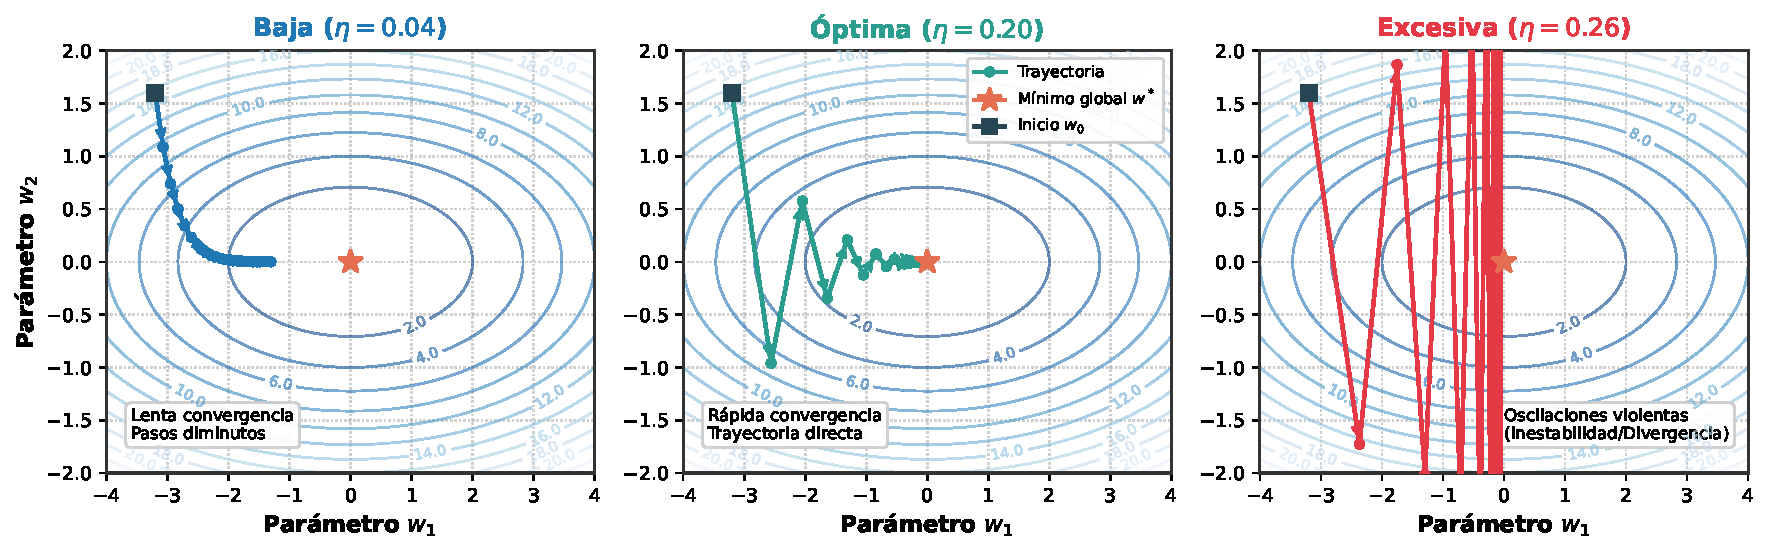
\includegraphics[width=0.88\textwidth]{fig1_learning_rate.pdf}
  \end{center}
  \vspace{-0.25cm}
  \begin{columns}[T]
    \begin{column}{0.32\textwidth}
      \textbf{Tasa Baja ($\eta = 0.04$)}
      \begin{itemize}\scriptsize
        \item Pasos diminutos en el gradiente.
        \item Convergencia lenta; riesgo de estancamiento en mesetas o mínimos locales planos.
      \end{itemize}
    \end{column}
    \begin{column}{0.34\textwidth}
      \textbf{Tasa Óptima ($\eta = 0.20$)}
      \begin{itemize}\scriptsize
        \item Descenso eficiente hacia el óptimo $\theta^*$.
        \item Teóricamente $\eta_{\text{ópt}} = \frac{2}{\lambda_{\max} + \lambda_{\min}}$ en cuencas parabólicas.
      \end{itemize}
    \end{column}
    \begin{column}{0.32\textwidth}
      \textbf{Tasa Excesiva ($\eta = 0.26$)}
      \begin{itemize}\scriptsize
        \item ``Overshooting'' y rebote entre paredes opuestas de la cuenca.
        \item Inestabilidad numérica, oscilaciones y divergencia a $\infty$ o NaN.
      \end{itemize}
    \end{column}
  \end{columns}
\end{frame}

% -----------------------------------------------------------------------------
% SLIDE 5: ESCALADO DE CARACTERÍSTICAS (STANDARD SCALER)
% -----------------------------------------------------------------------------
\begin{frame}{Parámetro 2: Escalado de Datos y Condicionamiento del Hessiano}
  \begin{center}
    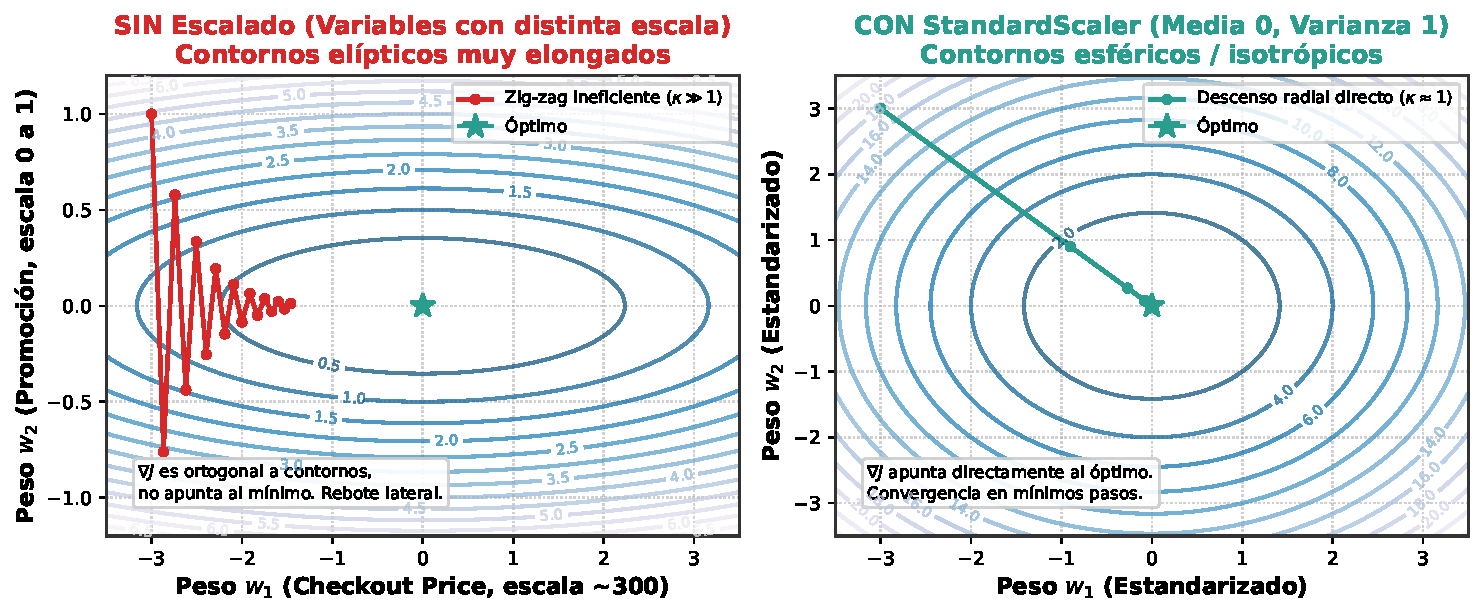
\includegraphics[width=0.80\textwidth]{fig2_scaling.pdf}
  \end{center}
  \vspace{-0.3cm}
  \begin{columns}[T]
    \begin{column}{0.48\textwidth}
      \textbf{¿Por qué ocurre el Zig-Zag sin Escalar?}
      \begin{itemize}\scriptsize
        \item \texttt{checkout\_price} $\sim 300$, mientras \texttt{emailer} $\in \{0, 1\}$.
        \item Número de condición $\kappa(H) = \frac{\lambda_{\max}}{\lambda_{\min}} \gg 1$.
        \item El vector gradiente $\nabla J$ es ortogonal a las curvas de nivel, apuntando casi perpendicular al mínimo; genera rebotes laterales inútiles.
      \end{itemize}
    \end{column}
    \begin{column}{0.48\textwidth}
      \textbf{Efecto de \texttt{StandardScaler} ($z = \frac{x - \mu}{\sigma}$)}
      \begin{itemize}\scriptsize
        \item Lleva la varianza de cada variable a $1.0$ y la media a $0$.
        \item Esferifica las curvas de nivel ($\kappa(H) \approx 1$).
        \item El gradiente apunta \textbf{directamente al mínimo teórico}, permitiendo pasos amplios y acelerando drásticamente el aprendizaje.
      \end{itemize}
    \end{column}
  \end{columns}
\end{frame}

% -----------------------------------------------------------------------------
% SLIDE 6: TAMAÑO DE LOTE (BATCH SIZE)
% -----------------------------------------------------------------------------
\begin{frame}{Parámetro 3: Tamaño de Lote ($B$) — Ruido y Generalización}
  \begin{center}
    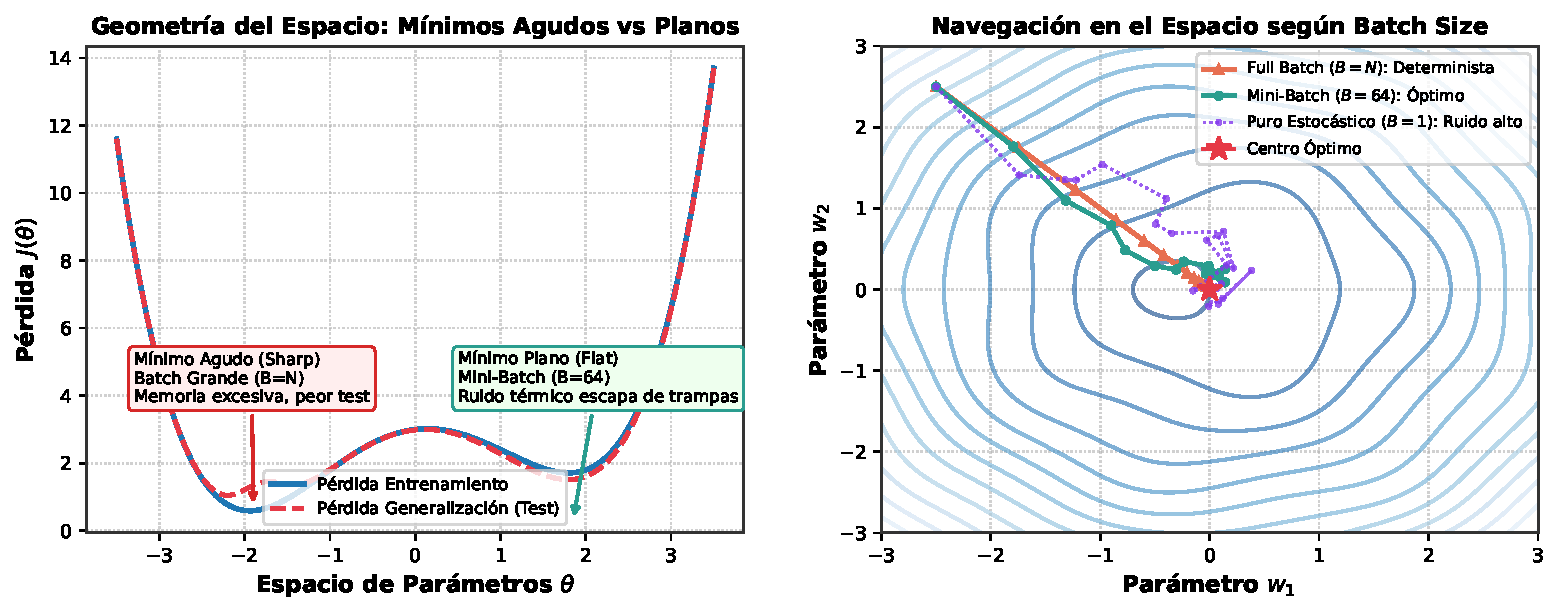
\includegraphics[width=0.82\textwidth]{fig3_batch_size.pdf}
  \end{center}
  \vspace{-0.3cm}
  \begin{columns}[T]
    \begin{column}{0.32\textwidth}
      \textbf{Lote Unitario ($B=1$, SGD puro)}
      \begin{itemize}\scriptsize
        \item Varianza máxima del gradiente: $\text{Var}(g_B) \propto 1/B$.
        \item Caminata errática; ineficiente en hardware moderno por falta de vectorización.
      \end{itemize}
    \end{column}
    \begin{column}{0.34\textwidth}
      \textbf{Mini-Batch ($B=64$, Punto Dulce)}
      \begin{itemize}\scriptsize
        \item Ruido térmico óptimo que permite \textbf{escapar de mínimos agudos (sharp minima)}.
        \item Converge a mínimos anchos (flat minima) que ofrecen \textbf{alta generalización}.
      \end{itemize}
    \end{column}
    \begin{column}{0.32\textwidth}
      \textbf{Batch Completo ($B=N$)}
      \begin{itemize}\scriptsize
        \item Gradiente determinista exacto.
        \item Alto consumo de memoria; tiende a atraparse en mínimos locales estrechos y sobreajustar.
      \end{itemize}
    \end{column}
  \end{columns}
\end{frame}

% -----------------------------------------------------------------------------
% SLIDE 7: NÚMERO DE ÉPOCAS Y SESGO-VARIANZA
% -----------------------------------------------------------------------------
\begin{frame}{Parámetro 4: Número de Épocas ($E$) — Dinámica Temporal}
  \begin{center}
    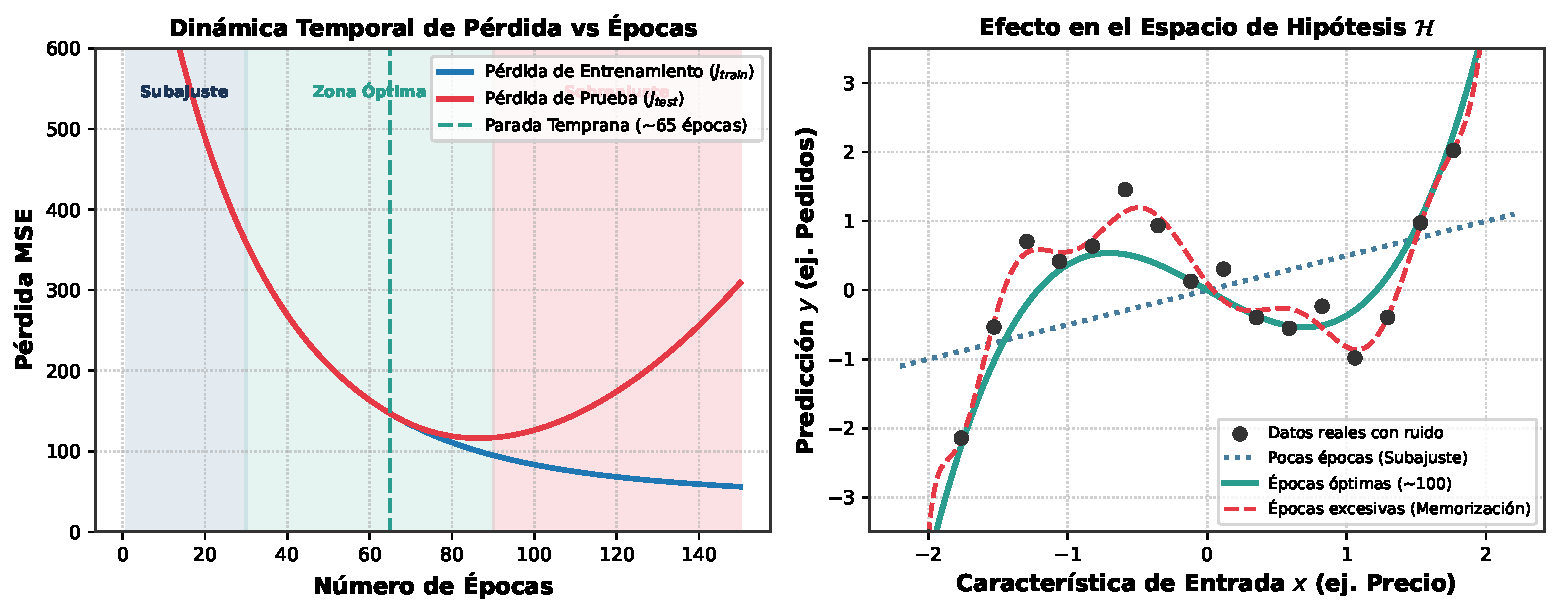
\includegraphics[width=0.82\textwidth]{fig4_epochs_overfitting.pdf}
  \end{center}
  \vspace{-0.3cm}
  \begin{columns}[T]
    \begin{column}{0.32\textwidth}
      \textbf{Pocas Épocas ($E < 30$): Subajuste}
      \begin{itemize}\scriptsize
        \item Alto sesgo (Underfitting).
        \item La red no ha alcanzado la cuenca de convergencia; predicciones planas o insuficientes.
      \end{itemize}
    \end{column}
    \begin{column}{0.34\textwidth}
      \textbf{Épocas Óptimas ($E \approx 100$)}
      \begin{itemize}\scriptsize
        \item Punto de equilibrio donde el error de prueba $J_{\text{test}}$ alcanza su mínimo.
        \item Captura la señal real subyacente sin memorizar el ruido muestral.
      \end{itemize}
    \end{column}
    \begin{column}{0.32\textwidth}
      \textbf{Épocas Excesivas ($E > 150$): Sobreajuste}
      \begin{itemize}\scriptsize
        \item Alta varianza (Overfitting).
        \item $J_{\text{train}} \to 0$ mientras $J_{\text{test}}$ diverge.
        \item La red ajusta oscilaciones espurias interpolando ruido de la muestra.
      \end{itemize}
    \end{column}
  \end{columns}
\end{frame}

% -----------------------------------------------------------------------------
% SLIDE 8: ARQUITECTURA (CAPAS Y NEURONAS)
% -----------------------------------------------------------------------------
\begin{frame}{Parámetro 5: Arquitectura — Capacidad del Espacio de Hipótesis}
  \begin{center}
    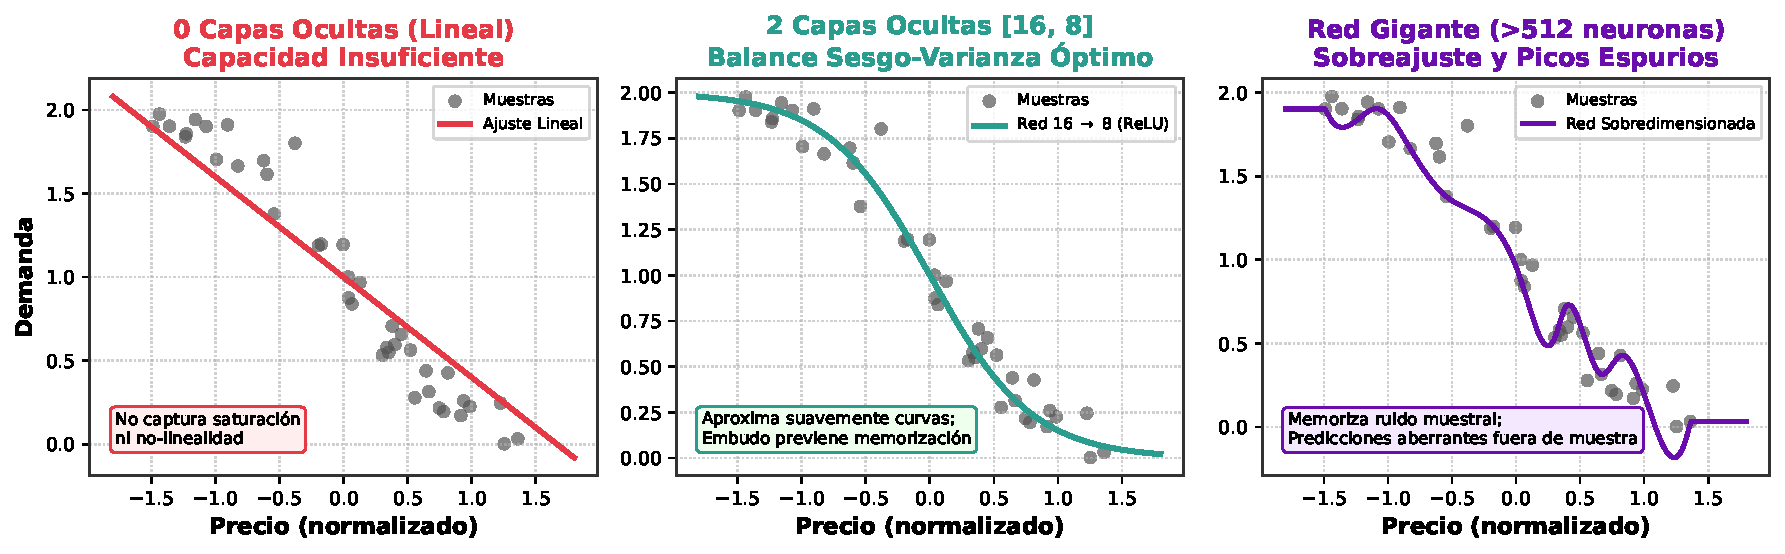
\includegraphics[width=0.85\textwidth]{fig5_architecture.pdf}
  \end{center}
  \vspace{-0.3cm}
  \begin{columns}[T]
    \begin{column}{0.32\textwidth}
      \textbf{0 Capas Ocultas (Lineal)}
      \begin{itemize}\scriptsize
        \item $\hat{y} = Wx + b$.
        \item Espacio rígido; no modela la interacción no lineal precio--promoción ni la saturación de demanda.
      \end{itemize}
    \end{column}
    \begin{column}{0.34\textwidth}
      \textbf{2 Capas [$16 \to 8$] (Embudo)}
      \begin{itemize}\scriptsize
        \item $5 \to 16 \to 8 \to 1$ ($241$ pesos).
        \item El embudo comprime representaciones abstractas; previene memorización y aproxima curvas suaves.
      \end{itemize}
    \end{column}
    \begin{column}{0.32\textwidth}
      \textbf{Red Sobredimensionada ($>512$ n)}
      \begin{itemize}\scriptsize
        \item Miles de parámetros vs. $1600$ datos.
        \item Espacio de hipótesis gigante: mínimos espurios y predicciones aberrantes fuera de muestra.
      \end{itemize}
    \end{column}
  \end{columns}
\end{frame}

% -----------------------------------------------------------------------------
% SLIDE 9: FUNCIÓN DE ACTIVACIÓN (RELU vs LINEAL vs SIGMOIDE)
% -----------------------------------------------------------------------------
\begin{frame}{Parámetro 6: Función de Activación — No Linealidad y Gradientes}
  \begin{center}
    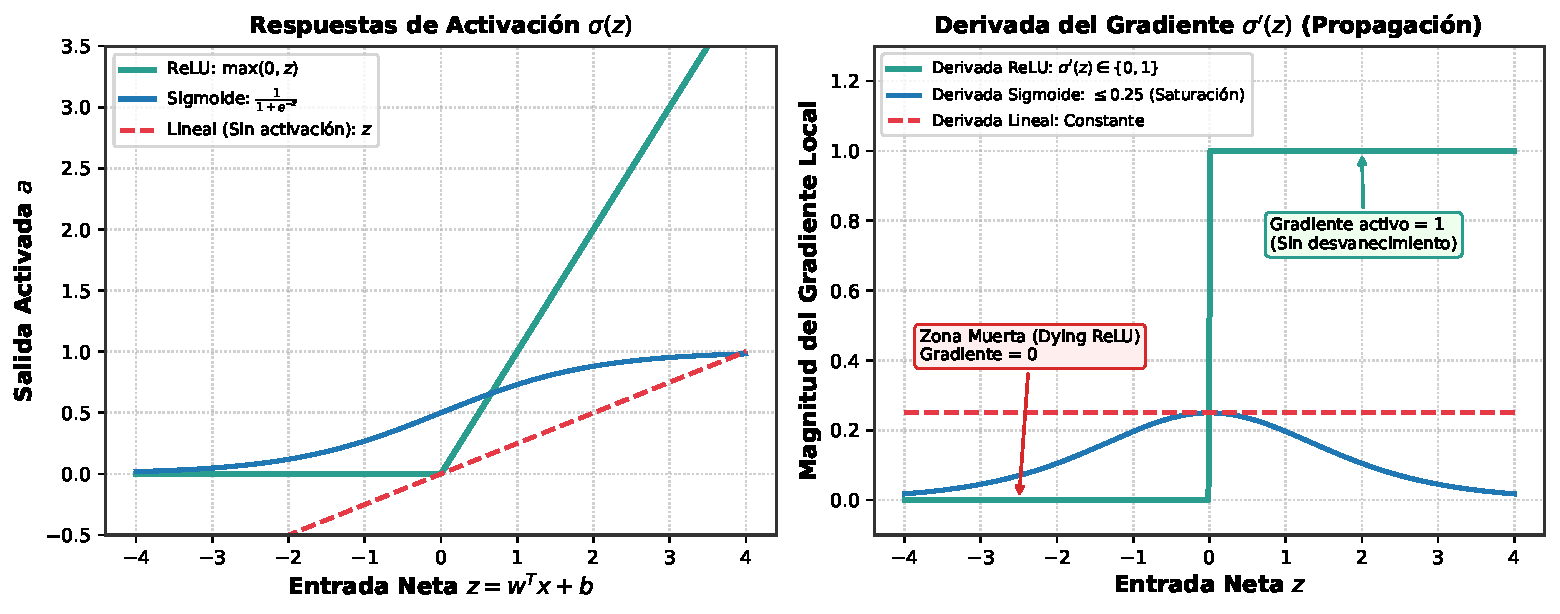
\includegraphics[width=0.82\textwidth]{fig6_activations.pdf}
  \end{center}
  \vspace{-0.3cm}
  \begin{columns}[T]
    \begin{column}{0.32\textwidth}
      \textbf{Lineal: Colapso Matemático}
      \begin{itemize}\scriptsize
        \item $W_2(W_1 x + b_1) + b_2 = (W_2 W_1)x + b'$.
        \item Apilar capas lineales colapsa a una única matriz afín; anula la profundidad.
      \end{itemize}
    \end{column}
    \begin{column}{0.34\textwidth}
      \textbf{Sigmoide / Tanh: Saturación}
      \begin{itemize}\scriptsize
        \item $\sigma'(z) \le 0.25$.
        \item Por regla de la cadena: $\prod_{l=1}^L \sigma' \to 0$.
        \item Desvanecimiento del gradiente en capas iniciales (Vanishing Gradient).
      \end{itemize}
    \end{column}
    \begin{column}{0.32\textwidth}
      \textbf{ReLU: Gradiente Robusto}
      \begin{itemize}\scriptsize
        \item $\sigma'(z) = 1$ para $z > 0$.
        \item Flujo de gradiente limpio sin atenuación; cálculo algebraico ultra veloz.
        \item \textit{Salida sin activación}: Codominio libre $\mathbb{R}$ para regresión continua.
      \end{itemize}
    \end{column}
  \end{columns}
\end{frame}

% -----------------------------------------------------------------------------
% SLIDE 10: OPTIMIZADOR (ADAM vs SGD vs MOMENTUM)
% -----------------------------------------------------------------------------
\begin{frame}{Parámetro 7: Optimizador — Cinemática Adaptativa en el Paisaje}
  \begin{columns}[c]
    \begin{column}{0.48\textwidth}
      \begin{center}
        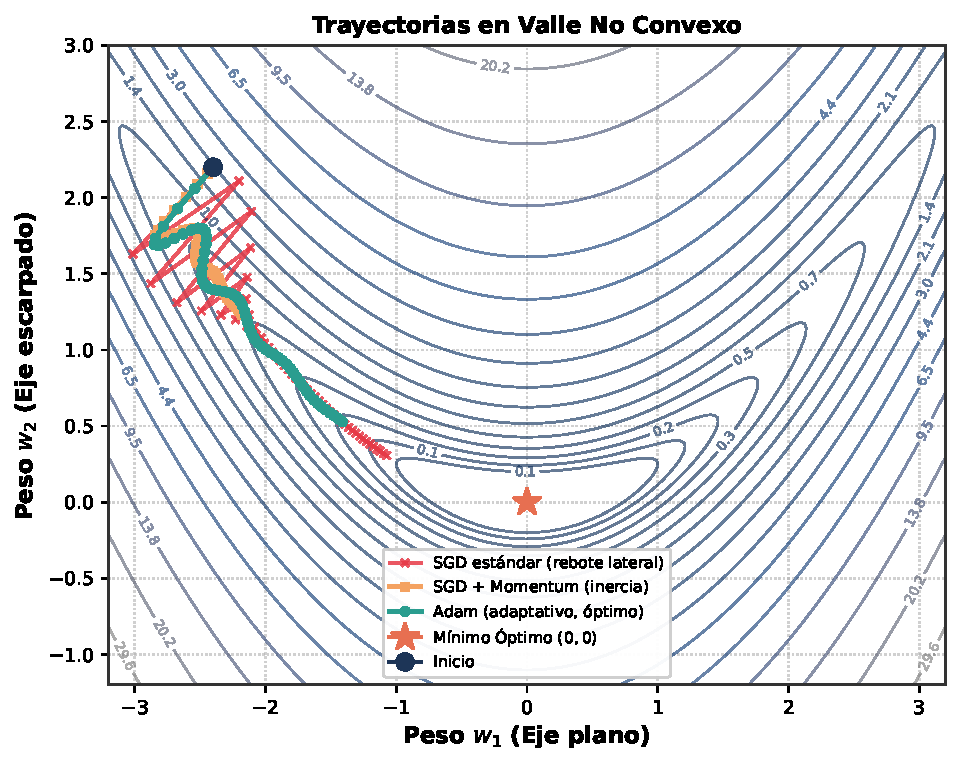
\includegraphics[width=0.98\linewidth]{fig7_optimizers.pdf}
      \end{center}
    \end{column}

    \begin{column}{0.50\textwidth}
      \textbf{Mecánica de Adam (Adaptive Moments)}
      \begin{itemize}\scriptsize
        \item $m_t = \beta_1 m_{t-1} + (1-\beta_1) g_t$ \quad (1º Momento / Inercia)
        \item $v_t = \beta_2 v_{t-1} + (1-\beta_2) g_t^2$ \quad (2º Momento / Curvatura)
        \item $\theta_{t+1} = \theta_t - \frac{\eta}{\sqrt{\hat{v}_t} + \epsilon} \hat{m}_t$
      \end{itemize}

      \vspace{0.1cm}
      \textbf{Dinámica en Gargantas Estrechas y Valles}
      \begin{itemize}\scriptsize
        \item \textbf{SGD estándar}: Sufre en paisajes anisótropos. Da pasos gigantescos en la dirección escarpada y pasos minúsculos en la dirección longitudinal plana.
        \item \textbf{SGD + Momentum}: Acumula inercia en la dirección persistente y cancela oscilaciones transversales.
        \item \textbf{Adam (\texttt{red\_neuronal.py})}: Normaliza el paso por parámetro dividiendo por $\sqrt{v_t}$. Avanza con paso firme y rápido en direcciones planas sin desestabilizarse.
      \end{itemize}
    \end{column}
  \end{columns}
\end{frame}

% -----------------------------------------------------------------------------
% SLIDE 11: FUNCIÓN DE PÉRDIDA (MSE vs MAE vs HUBER)
% -----------------------------------------------------------------------------
\begin{frame}{Parámetro 8: Función de Pérdida — Geometría del Error y Robustez}
  \begin{center}
    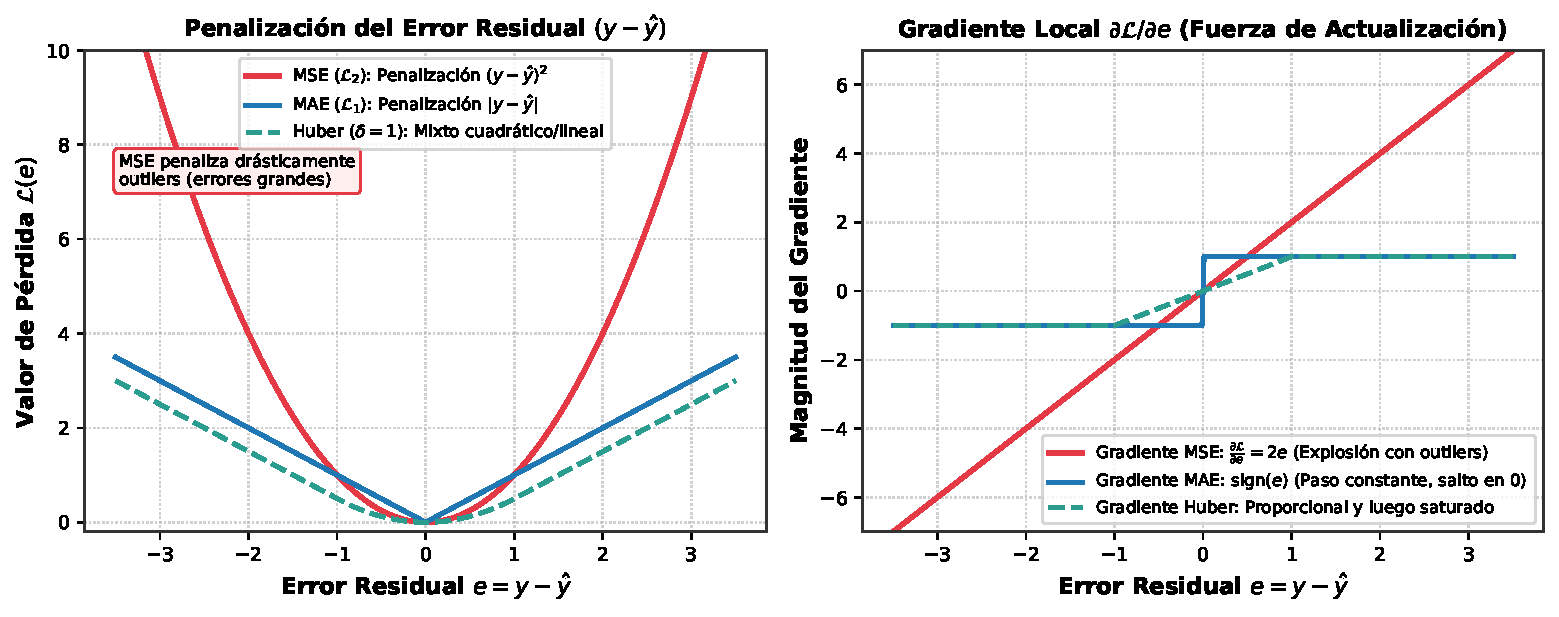
\includegraphics[width=0.82\textwidth]{fig8_loss_functions.pdf}
  \end{center}
  \vspace{-0.3cm}
  \begin{columns}[T]
    \begin{column}{0.48\textwidth}
      \textbf{Error Cuadrático Medio (\texttt{MSELoss}, $L_2$)}
      \begin{itemize}\scriptsize
        \item $\mathcal{L}_{MSE} = (y - \hat{y})^2 \implies \nabla = 2(y - \hat{y})$.
        \item Cuenca parabólica suave: gradiente proporcional al error; garantiza convergencia precisa y estable cerca del mínimo.
        \item \textit{Riesgo}: Errores atípicos (outliers de demanda extrema) generan gradientes muy grandes que pueden perturbar el aprendizaje.
      \end{itemize}
    \end{column}
    \begin{column}{0.48\textwidth}
      \textbf{Error Absoluto Medio (\texttt{L1Loss}, MAE)}
      \begin{itemize}\scriptsize
        \item $\mathcal{L}_{MAE} = |y - \hat{y}| \implies \nabla = \text{sign}(y - \hat{y})$.
        \item Gradiente constante e inmune a valores extremos (robusto a outliers).
        \item \textit{Desventaja}: Discontinuidad del gradiente en $0$; tiende a oscilar alrededor del mínimo si la tasa $\eta$ no decae asintóticamente.
      \end{itemize}
    \end{column}
  \end{columns}
\end{frame}

% -----------------------------------------------------------------------------
% SLIDE 12: MATRIZ DE INTERACCIÓN Y CO-DISEÑO
% -----------------------------------------------------------------------------
\begin{frame}{Interacción y Reglas de Co-diseño entre Hiperparámetros}
  Los parámetros libres no operan de forma aislada; interactúan en el espacio de solución:
  \vspace{0.15cm}

  \begin{center}
    \scriptsize
    \begin{tabular}{p{2.8cm} p{3.2cm} p{5.8cm}}
      \toprule
      \textbf{Si modificas...} & \textbf{Efecto Secundario} & \textbf{Ajuste Compensatorio Recomendado} \\
      \midrule
      Aumentar \textbf{Batch Size ($B$)} & Reduce el ruido de gradiente & \textbf{Aumentar $\eta$} proporcionalmente (Regla de escala lineal $\eta \propto B$). \\
      \addlinespace
      Aumentar \textbf{Capas / Ancho} & Expande $\mathcal{H}$ y riesgo de sobreajuste & \textbf{Reducir Épocas} o agregar regularización ($L_2$ \texttt{weight\_decay} o \texttt{Dropout}). \\
      \addlinespace
      Cambiar de \textbf{Adam a SGD} & Pierde adaptabilidad de curvatura & \textbf{Añadir Momentum} ($\beta=0.9$) y usar un planificador de tasa (\texttt{Scheduler}). \\
      \addlinespace
      Eliminar \textbf{StandardScaler} & Elipses de pérdida $\kappa(H) \gg 1$ & \textbf{Reducir drásticamente $\eta$} para evitar divergencia, a costa de convergencia lenta. \\
      \addlinespace
      Aumentar \textbf{Épocas ($E > 200$)} & Memorización asintótica & Implementar \textbf{Early Stopping} monitoreando la pérdida de validación. \\
      \bottomrule
    \end{tabular}
  \end{center}
\end{frame}

% -----------------------------------------------------------------------------
% SLIDE 13: CONCLUSIONES Y GUÍA PRÁCTICA
% -----------------------------------------------------------------------------
\begin{frame}{Conclusiones y Guía Práctica de Ajuste}
  \begin{columns}[T]
    \begin{column}{0.48\textwidth}
      \begin{block}{Principios del Espacio Teórico}
        \scriptsize
        \begin{itemize}
          \item La \textbf{geometría del paisaje} está determinada por el preprocesamiento, la arquitectura y la pérdida.
          \item La \textbf{cinemática de la trayectoria} está controlada por el optimizador, la tasa $\eta$ y el batch size $B$.
          \item El objetivo no es minimizar a ciegas $J_{\text{train}}$, sino encontrar un \textbf{mínimo plano generalizable}.
        \end{itemize}
      \end{block}
    \end{column}

    \begin{column}{0.48\textwidth}
      \begin{alertblock}{Protocolo de Diagnóstico en \texttt{red\_neuronal.py}}
        \scriptsize
        \begin{itemize}
          \item \textbf{¿Pérdida es NaN o explota?} $\implies$ Disminuir $\eta$ o verificar escalado de datos.
          \item \textbf{¿Aprende demasiado lento?} $\implies$ Aumentar $\eta$ o verificar que no haya neuronas muertas (Dying ReLU).
          \item \textbf{¿$R^2$ alto en Train pero bajo en Test?} $\implies$ Sobreajuste: reducir épocas o simplificar arquitectura ($16 \to 8$).
          \item \textbf{¿$R^2$ bajo en ambos?} $\implies$ Subajuste: verificar activación y añadir capacidad.
        \end{itemize}
      \end{alertblock}
    \end{column}
  \end{columns}
\end{frame}

% -----------------------------------------------------------------------------
% SLIDE 14: CIERRE
% -----------------------------------------------------------------------------
\begin{frame}[standout]
  \Huge ¿Preguntas o Discusión?
  \vspace{0.4cm}

  \normalsize Código fuente de referencia: \texttt{red\_neuronal.py} \\
  Gráficas generadas con Matplotlib (Vector PDF)
\end{frame}

\end{document}
